\documentclass[twoside]{article}

\usepackage[preprint]{aistats2026}
\usepackage[utf8]{inputenc}
\usepackage[T1]{fontenc}
\usepackage{natbib}
\usepackage{hyperref}
\hypersetup{hidelinks}
\usepackage{booktabs}
\usepackage{adjustbox}
\usepackage{amsmath,amssymb,amsthm,amsfonts,mathtools}
\usepackage{graphicx}
\usepackage{subcaption}
\usepackage{float}
\captionsetup[subfigure]{font=footnotesize,justification=centering,singlelinecheck=false}
\usepackage{xcolor}
\usepackage{enumitem}
\usepackage{tikz}
\usetikzlibrary{arrows.meta,positioning,fit,backgrounds,shapes}

\newtheorem{theorem}{Theorem}
\newtheorem{definition}{Definition}
\newtheorem{proposition}{Proposition}
\newtheorem{corollary}{Corollary}
\newtheorem{lemma}{Lemma}
\newtheorem{assumption}{Assumption}
\newtheorem{remark}{Remark}

\newcommand{\R}{\mathbb{R}}
\newcommand{\E}{\mathbb{E}}
\newcommand{\doo}{\mathrm{do}}
\newcommand{\An}{\mathrm{An}}
\newcommand{\QCBO}{\textsc{QCBO}}
\newcommand{\HQCBO}{\textsc{HQCBO}}
\newcommand{\QDCBO}{\textsc{QDCBO}}
\newcommand{\QMCBO}{\textsc{QMCBO}}
\newcommand{\CBO}{\textsc{CBO}}
\newcommand{\Gg}{\mathcal{G}}
\newcommand{\Gq}{\mathcal{G}^{\Pi}}
\newcommand{\ES}{\mathbf{ES}}
\newcommand{\ESpi}{\mathbf{ES}^{\Pi}}

\definecolor{okorange}{HTML}{E69F00}
\definecolor{okblue}{HTML}{56B4E9}
\definecolor{okpurple}{HTML}{CC79A7}
\tikzset{
  obsnode/.style={circle,draw=black!75,minimum size=6.5mm,inner sep=1pt,font=\small},
  mannode/.style={obsnode,fill=okorange!45},
  tgtnode/.style={obsnode,fill=okblue!45},
  clbox/.style={draw=black!55,dashed,rounded corners,inner sep=3.2mm},
  diredge/.style={->,>=Stealth,semithick,black!80},
  bicross/.style={<->,>=Stealth,okpurple,dashdotted,semithick},
  biintra/.style={bicross},
}

\begin{document}

\runningtitle{Coarsening Confers Robustness in Causal Bayesian Optimization}
\runningauthor{Anonymous}

\twocolumn[
\aistatstitle{Coarsening Confers Robustness: \\
Causal Bayesian Optimization under Directed Acyclic Graph Misspecification}
\aistatsauthor{Anonymous}
\aistatsaddress{Anonymous}
]

\begin{abstract}
\end{abstract}

\section{Introduction}
\label{sec:intro}

Causal Bayesian optimization (CBO)
\citep{agliettiCausalBayesianOptimization2020b} searches for an intervention
that optimizes a target while using observational data to reduce the number
of costly experiments. Its assumed causal graph determines which
intervention sets are considered and which causal effects can be used as
prior means. A misspecified graph can consequently do more than slow
learning: it can exclude the best intervention from the search space.

\begin{figure}[t]
  \centering
  % Motivating example (Fig. 1): three semantic subfigures.
\begin{subfigure}[t]{0.32\linewidth}
  \centering
  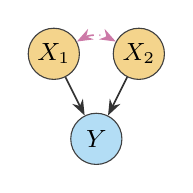
\begin{tikzpicture}[x=0.72cm,y=0.72cm]
    \node[mannode] (X1) at (0,1.15) {$X_1$};
    \node[mannode] (X2) at (1.5,1.15) {$X_2$};
    \node[tgtnode] (Y) at (0.75,-0.35) {$Y$};
    \draw[diredge] (X1) -- (Y);
    \draw[diredge] (X2) -- (Y);
    \draw[bicross] (X1) to[bend left=28] (X2);
  \end{tikzpicture}
  \caption{True graph}
  \label{fig:motivating-true}
\end{subfigure}\hfill
\begin{subfigure}[t]{0.32\linewidth}
  \centering
  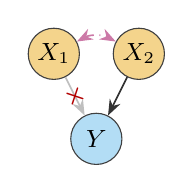
\begin{tikzpicture}[x=0.72cm,y=0.72cm]
    \node[mannode] (X1) at (0,1.15) {$X_1$};
    \node[mannode] (X2) at (1.5,1.15) {$X_2$};
    \node[tgtnode] (Y) at (0.75,-0.35) {$Y$};
    \draw[diredge,black!25] (X1) -- (Y)
      node[midway,sloped] {\textcolor{red!70!black}{\footnotesize$\boldsymbol{\times}$}};
    \draw[diredge] (X2) -- (Y);
    \draw[bicross] (X1) to[bend left=28] (X2);
  \end{tikzpicture}
  \caption{Assumed graph}
  \label{fig:motivating-assumed}
\end{subfigure}\hfill
\begin{subfigure}[t]{0.32\linewidth}
  \centering
  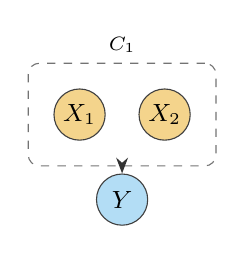
\begin{tikzpicture}[x=0.72cm,y=0.72cm]
    \node[mannode] (X1) at (0,1.15) {$X_1$};
    \node[mannode] (X2) at (1.5,1.15) {$X_2$};
    \node[tgtnode] (Y) at (0.75,-0.35) {$Y$};
    \begin{scope}[on background layer]
      \node[clbox,fit=(X1)(X2),label={[font=\scriptsize]above:$C_1$}] (C1) {};
    \end{scope}
    \draw[diredge] (C1.south) -- (Y);
  \end{tikzpicture}
  \caption{Common quotient}
  \label{fig:motivating-quotient}
\end{subfigure}

  \caption{The \textsc{ParallelParent} construction. Deleting
  $X_1\to Y$ changes the fine exploration set but not the quotient because
  the cluster edge $C_1\to Y$ remains through $X_2\to Y$. Orange nodes are
  manipulable, blue is the target, and the dash-dotted edge denotes latent
  confounding.}
  \label{fig:motivating}
\end{figure}

Figure~\ref{fig:motivating} illustrates the failure mode. The confounded
parents $X_1$ and $X_2$ jointly determine $Y$, and the optimum requires
setting both variables. If the hypothesis graph deletes $X_1\to Y$, the
fine-graph optimizer discards every intervention containing $X_1$. If the
two variables are instead represented by the cluster
$C_1=\{X_1,X_2\}$, the edge $C_1\to Y$ survives through $X_2\to Y$ and
the whole-cluster intervention remains available.

This observation motivates a deliberate change of resolution. QCBO receives
a partition and its quotient graph as inputs and restricts interventions to
unions of manipulable clusters. Such clusters may encode a known subsystem,
a policy module, or another domain-defined unit whose coarse causal
relationships are more reliable than its internal structure. The present
work does not learn the partition or the quotient graph. Coarsening removes
sensitivity to distinctions within clusters, but it can also hide useful
fine-grained actions.

Our contributions are threefold. First, we formalize the \emph{quotient
contract}: every graph-dependent component of the optimizer factors through
the quotient. This yields exact trajectory invariance over the class of fine
graphs with the same quotient and a worst-case regret separation from
fine-graph methods. Second, we characterize the price of restricting the
action space to cluster unions, establish monotonicity under refinement, and
give structural conditions for zero price. Third, we instantiate the
contract for arm-based, dynamic, and model-based causal Bayesian optimizers
and evaluate the predicted invariances and trade-offs. Proofs, complete
dataset graphs, and additional results are provided in the appendices.

\section{Problem setup and quotient construction}
\label{sec:setup}

\subsection{Causal Bayesian optimization}

Let
$\mathcal M=\langle\mathbf U,\mathbf V,F,P(\mathbf U)\rangle$ be a fixed
structural causal model (SCM) with target $Y\in\mathbf V$ and manipulable
variables $\mathbf X\subseteq\mathbf V$ \citep{pearlCausality2009}. Its
latent projection is an acyclic directed mixed graph (ADMG) $\Gg$ whose
directed edges represent causal relations and whose bidirected edges
represent latent confounding. Throughout, population expectations and
intervention outcomes are defined by this fixed true SCM. A hypothesis graph
supplied to an optimizer can change its decisions, but never the
data-generating distribution.

An intervention arm is a nonempty set $A\subseteq\mathbf X$. Let $D(A)$
denote the Cartesian intervention domain for the variables in $A$. For
minimization,
the population value of an arm is
\begin{equation}
  \mu^\star(A):=\min_{a\in D(A)}
  \E_{\mathcal M}\!\left[Y\mid\doo(A=a)\right].
  \label{eq:arm-value}
\end{equation}
CBO maintains a Gaussian process (GP) for each retained arm. Its exploration
set consists of the graph's minimal intervention sets (MIS)
\citep{leeStructuralCausalBandits,agliettiCausalBayesianOptimization2020b}.
Writing $\Gg_{\bar A}$ for the graph obtained by deleting incoming edges to
$A$, the MIS are
\begin{equation}
  \ES(\Gg)=\mathrm{MIS}(\Gg)
  :=\left\{A\subseteq\mathbf X:
  \substack{A\ne\emptyset,\\
  A\subseteq\An(Y)\text{ in }\Gg_{\bar A}}\right\}.
  \label{eq:mis}
\end{equation}
For every retained arm $A$, CBO places a GP prior on the interventional
response surface
\begin{equation}
  f_A(a):=\E_{\mathcal M}[Y\mid\doo(A=a)],
  \qquad f_A\sim\mathcal{GP}(m_A^H,k_A).
  \label{eq:cbo-gp}
\end{equation}
The prior mean is a plug-in estimate of the causal effect whenever that
effect is identified under the hypothesis graph $H$. In particular, if a
complete identification procedure returns the functional
\begin{equation}
  p_H(y\mid\doo(A=a))=\mathfrak I_A^H(p)(y;a),
  \label{eq:id-functional}
\end{equation}
then, for an estimate $\widehat p$ of the observational distribution,
\begin{equation}
  m_A^H(a)=\int y\,\mathfrak I_A^H(\widehat p)(y;a)\,\mathrm dy.
  \label{eq:causal-prior}
\end{equation}
For example, if $Z$ is a valid adjustment set, this reduces to the familiar
backdoor estimator
\begin{equation}
  m_A^H(a)=\int \widehat{\E}[Y\mid A=a,Z=z]\,\mathrm d\widehat P(z).
  \label{eq:backdoor-prior}
\end{equation}
Under causal sufficiency, the truncated factorization provides the
$g$-computation functional
\begin{equation}
  \widehat p(v\setminus a\mid\doo(a))
  =\prod_{V_i\in\mathbf V\setminus A}
    \widehat p(v_i\mid\operatorname{pa}_i),
  \label{eq:g-formula}
\end{equation}
which is integrated against $Y$ to obtain Equation~\eqref{eq:causal-prior}.
Equation~\eqref{eq:g-formula} is one identified functional, not a substitute
for complete identification in an ADMG; frontdoor and more general
functionals may instead be required.

Let $K_{A,t}$ be the kernel matrix of the intervention values in
$\mathcal D_{A,t}$, $k_{A,t}(a)$ the vector of covariances between those
values and $a$, and $\mathbf y_{A,t}$ their observed outcomes. Define
$C_{A,t}:=K_{A,t}+\sigma_{A,\epsilon}^2I$ for independent Gaussian
observation noise of variance $\sigma_{A,\epsilon}^2$. The arm-wise GP
posterior is
\begin{align}
 \mu_{A,t}(a)
 &=m_A^H(a)+k_{A,t}(a)^\top
   C_{A,t}^{-1}(\mathbf y_{A,t}-\mathbf m_{A,t}^H),\nonumber\\
 \sigma_{A,t}^2(a)
 &=k_A(a,a)-k_{A,t}(a)^\top
   C_{A,t}^{-1}k_{A,t}(a),
 \label{eq:gp-posterior}
\end{align}
where $\mathbf m_{A,t}^H$ evaluates the causal prior mean at the observed
intervention values. For minimization, expected improvement over the
incumbent $y_t^{\mathrm{best}}$ is
\begin{align}
 z_{A,t}(a)&=\frac{y_t^{\mathrm{best}}-\mu_{A,t}(a)}
                   {\sigma_{A,t}(a)},\nonumber\\
 \operatorname{EI}_{A,t}(a)
 &=\bigl(y_t^{\mathrm{best}}-\mu_{A,t}(a)\bigr)
   \Phi(z_{A,t}(a))\nonumber\\
 &\quad+\sigma_{A,t}(a)\phi(z_{A,t}(a)),
 \label{eq:ei}
\end{align}
with the deterministic limit used when $\sigma_{A,t}(a)=0$. CBO selects the
arm and value maximizing $\operatorname{EI}_{A,t}(a)/c(A,a)$, where
$c(A,a)$ is the intervention cost. A common alternative is GP-UCB
\citep{srinivasGaussianProcessOptimization2010}:
\begin{align}
 \operatorname{UCB}_{A,t}(a)
 &=\mu_{A,t}(a)+\sqrt{\beta_t}\sigma_{A,t}(a),\nonumber\\
 \operatorname{LCB}_{A,t}(a)
 &=\mu_{A,t}(a)-\sqrt{\beta_t}\sigma_{A,t}(a),
 \label{eq:confidence-bounds}
\end{align}
where UCB is maximized and LCB is minimized. Our arm-based CBO and QCBO
experiments use cost-normalized EI; the model-based experiments retain the
base MCBO implementation's GP-UCB rule. More generally, each quotient method
preserves the acquisition rule of its base optimizer.

Thus an assumed graph $H$ enters CBO through
\begin{equation}
 H\longmapsto
 \left(\ES(H),\{m_A^H\}_{A\in\ES(H)}\right)
 \longmapsto \tau_{\mathcal A}(H),
 \label{eq:trajectory-map}
\end{equation}
where $m_A^H$ is the prior-mean function computed under $H$ and
$\tau_{\mathcal A}(H)$ is the complete optimization trajectory: selected
arms, intervention values, observations, and incumbents.

\subsection{Quotients and cluster-union interventions}

For a partition $\Pi$ of $\mathbf V$, let $\chi:\mathbf V\to\Pi$ map each
variable to its cluster. The quotient $\Gg^\Pi$ has a directed edge
$\chi(u)\to\chi(v)$ whenever $u\to v$ is present in $\Gg$ and
$\chi(u)\ne\chi(v)$; bidirected edges are mapped analogously. The partition
is \emph{valid} when the directed quotient is acyclic, and we write
\begin{equation}
  Q_\Pi(\Gg):=(\Pi,\Gg^\Pi).
  \label{eq:quotient}
\end{equation}
We assume that every cluster intersecting $\mathbf X$ is wholly manipulable;
all other variables may remain singleton clusters. Let
$\Pi_M:=\{C\in\Pi:C\subseteq\mathbf X\}$ denote the manipulable clusters.
The action family available at resolution $\Pi$ is
\begin{equation}
  \mathcal U(\Pi)=
  \left\{\bigcup_{C\in S}C:\emptyset\ne S\subseteq\Pi_M\right\}.
  \label{eq:cluster-actions}
\end{equation}
QCBO applies the MIS rule to the quotient and expands each selected cluster
arm to its constituent variables.

Let $\Pi_\bot:=\{\{v\}:v\in\mathbf V\}$ denote the singleton partition.
The best population value reachable under $\Pi$ and its loss relative to
the full fine action space are
\begin{equation}
  V(\Pi):=\min_{A\in\mathcal U(\Pi)}\mu^\star(A),
  \qquad
  \Delta(\Pi):=V(\Pi)-V(\Pi_\bot).
  \label{eq:price}
\end{equation}
We call $\Delta(\Pi)$ the \emph{price of coarsening}. For minimization it is
nonnegative. It measures the loss caused by the restricted action space. For
example, if $\Pi$ contains the manipulable cluster $\{X_1,X_2\}$, then the
fine action family contains $\{X_1\}$, $\{X_2\}$, and
$\{X_1,X_2\}$, whereas the coarse family contains only
$\{X_1,X_2\}$.

For an incumbent intervention $\hat a_t$ after trial $t$, let
$\mu(\hat a_t)$ be its expected outcome under the true SCM and define
\begin{equation}
  y^\star:=V(\Pi_\bot),\qquad
  r_t:=\mu(\hat a_t)-y^\star,\qquad
  R_T:=\sum_{t=1}^{T}r_t.
  \label{eq:regret}
\end{equation}

\section{Robustness and the price of coarsening}
\label{sec:theory}

\subsection{Quotient invariance}
\label{sec:invariance}

For an ADMG $\Gg$ and valid partition $\Pi$, define the protected class
\begin{equation}
  E_\Pi(\Gg):=
  \left\{H:\substack{H\text{ is an ADMG over }\mathbf V,\\
  Q_\Pi(H)=Q_\Pi(\Gg)}\right\}.
  \label{eq:protected-class}
\end{equation}
This class contains within-cluster edits and cross-cluster edits that leave
every quotient edge represented. It excludes edits that add or remove a
quotient edge.

Let $\mathcal D$ denote the initial data, $\eta$ the hyperparameters, and
$\omega$ the optimizer's complete internal random stream (equivalently, its
random seed together with all subsequent random draws). The quotient
contract requires every graph-dependent operation to use a hypothesis graph
only through $Q_\Pi$. We write
$\mathcal A(H,\mathcal D,\omega,\eta)$ for a run of optimizer $\mathcal A$
under these inputs, and $\tau_{\mathcal A}(H;\mathcal D,\omega,\eta)$ for
the resulting sequence of selected arms, intervention values, observations,
and incumbents. In displays, let $\xi:=(\mathcal D,\omega,\eta)$.

\begin{proposition}[Exact quotient invariance]
\label{prop:contract}
Suppose
\[
 \mathcal A(H,\mathcal D,\omega,\eta)
 =\bar{\mathcal A}(Q_\Pi(H),\mathcal D,\omega,\eta).
\]
When two runs use the same true SCM, initial data, random stream, and
hyperparameters,
\[
 Q_\Pi(H)=Q_\Pi(H')
 \quad\Longrightarrow\quad
 \tau_{\mathcal A}(H;\xi)=\tau_{\mathcal A}(H';\xi).
\]
\end{proposition}

The two runs make the same first decision; because the true SCM is fixed,
they receive the same coupled observation; induction then gives identical
subsequent decisions and observations. In
Figure~\ref{fig:motivating}, deleting $X_1\to Y$ is protected because
$X_2\to Y$ preserves the quotient edge, whereas deleting both parent edges
removes $C_1\to Y$ and is not protected.

\subsection{Monotonicity under refinement}
\label{sec:price}

We write $\Pi'\preceq\Pi$ to mean that $\Pi'$ \emph{refines} $\Pi$: every
cluster of $\Pi'$ is contained in a cluster of $\Pi$. Refinement enlarges
the set of representable interventions.

\begin{proposition}[Monotonicity and price of coarsening]
\label{prop:price}
For valid $\Pi'\preceq\Pi$,
\[
 \mathcal U(\Pi)\subseteq\mathcal U(\Pi'),
 \qquad
 0\le\Delta(\Pi')\le\Delta(\Pi).
\]
Moreover,
\[
 \Delta(\Pi)=0
 \iff
 \arg\min_{A\in\mathcal U(\Pi_\bot)}\mu^\star(A)
 \cap\mathcal U(\Pi)\ne\emptyset.
\]
\end{proposition}

The result is purely about population reachability. Even when
$\Delta(\Pi)=0$, a partition can change intervention dimension, cost, arm
count, and finite-budget behavior.

\subsection{Sufficient conditions for lossless coarsening}
\label{sec:zero-price}

For $A\subseteq\mathbf X$, define its cluster closure and the variables
added by that closure as
\[
 \operatorname{cl}_\Pi(A):=\bigcup\{C\in\Pi:C\cap A\ne\emptyset\},
 \qquad B:=\operatorname{cl}_\Pi(A)\setminus A.
\]
For $a\in D(A)$, let $B_a$ denote the joint natural response of $B$ under
$\doo(A=a)$ and define
$D_B(a):=\{b:(a,b)\in D(\operatorname{cl}_\Pi(A))\}$.

\begin{proposition}[Sufficient conditions for zero price]
\label{prop:free}
Assume a semi-Markovian SCM. If, for every $A\subseteq\mathbf X$ and
$a\in D(A)$,
\begin{align*}
 \operatorname{supp}(B_a)&\subseteq D_B(a),\\
 B_a&\perp Y_{a,b}\quad\text{for every }b\in D_B(a),
\end{align*}
then $V(\Pi)=V(\Pi_\bot)$ and $\Delta(\Pi)=0$.
\end{proposition}

The first premise requires the intervention domain to contain the natural
responses that are replaced when the remainder of a cluster is clamped. The
second prevents the replacement from destroying a useful latent dependence
with the target. We state graph-level conditions that imply these premises.

\begin{definition}[Full intervention support]
\label{def:fullsupport}
Intervention domains are products,
$D(W)=\prod_{w\in W}D(w)$ for every $W\subseteq\mathbf X$, and for every
manipulable variable $v$ and intervention $a$ on
$A\subseteq\mathbf X\setminus\{v\}$,
$\operatorname{supp}(v_a)\subseteq D(v)$.
\end{definition}

\begin{definition}[Cluster-contained confounding]
\label{def:ccc}
Represent the semi-Markovian SCM by a nonparametric structural equation
model with mutually independent exogenous variables and augmented graph
$\Gg^{\mathrm{aug}}$. Here nonparametric means that the structural
mechanisms are not restricted to be linear, Gaussian, or members of a
specified finite-dimensional family. Semi-Markovian SCMs allow latent
confounding, represented by bidirected edges in the latent-projection ADMG,
and strictly generalize Markovian SCMs, which exclude such confounding. This
generality is needed for the confounded constructions studied in
Sections~\ref{sec:invariance} and~\ref{sec:experiments}. For
$A\subseteq\mathbf X$ and
$B=\operatorname{cl}_\Pi(A)\setminus A$, let $\mathbf U_B(A)$ be the
exogenous ancestors of $B$ after $\doo(A)$ and let $\mathbf U_Y(A)$ be the
exogenous ancestors of $Y$ after $\doo(\operatorname{cl}_\Pi(A))$. The
partition has cluster-contained confounding when
$\mathbf U_B(A)\cap\mathbf U_Y(A)=\emptyset$ for every
$A\subseteq\mathbf X$.
\end{definition}

\begin{corollary}[Graphical zero-price condition]
\label{cor:zero-price}
In a semi-Markovian SCM, full intervention support and cluster-contained
confounding imply $V(\Pi)=V(\Pi_\bot)$ and $\Delta(\Pi)=0$.
\end{corollary}

The condition is sufficient but not necessary. Because it constrains
counterfactual dependence across interventions, it is not generally
testable from a single observational or interventional distribution. It
should therefore be read as a structural guarantee supplied by domain
knowledge, rather than as a data-driven diagnostic.

\subsection{Protected-class regret separation}
\label{sec:separation}

Fix a true SCM $\mathcal M$ with graph $\Gg$. Outcomes are always generated
by $\mathcal M$, while the optimizer receives a hypothesis graph $H$. Let
$R_T(\mathcal A;H)$ denote the regret of a run using $H$ at fixed
$(\mathcal D,\omega,\eta)$. We denote worst-case regret over the protected
class by ``wc'':
\[
 R_T^{\mathrm{wc}}(\mathcal A;\Pi,\Gg)
 :=\sup_{H\in E_\Pi(\Gg)}R_T(\mathcal A;H).
\]
For a cluster-union incumbent, adding and subtracting the best value
available at resolution $\Pi$ gives
\begin{equation}
 \mu(\hat a_t)-y^\star
 =\underbrace{V(\Pi)-y^\star}_{\text{coarsening gap}}
 +\underbrace{\mu(\hat a_t)-V(\Pi)}_{\text{within-space optimization error}}.
 \label{eq:regret-decomposition}
\end{equation}
The first term is irreducible for a fixed action space and vanishes only
when $\Delta(\Pi)=0$. The second measures error relative to the best coarse
action and can converge to zero.

\begin{theorem}[Protected-class regret separation]
\label{thm:separation}
The following statements hold.
\begin{enumerate}[label=(\roman*),leftmargin=1.6em,itemsep=2pt,topsep=2pt]
  \item For every $\beta>0$, there exist a semi-Markovian SCM, a valid
  partition with $\Delta(\Pi)=0$, and a hypothesis
  $H\in E_\Pi(\Gg)$ obtained by deleting one directed edge, such that every
  optimizer whose initial and sequential interventions lie in
  $\mathrm{MIS}(H)$ and whose incumbent is selected among executed
  interventions satisfies
  \[
    r_t\ge\beta\quad\text{for every }t,
    \qquad R_T^{\mathrm{wc}}(\mathcal A;\Pi,\Gg)\ge\beta T.
  \]
  \item If an optimizer satisfies Proposition~\ref{prop:contract}, executes
  only cluster-union interventions, and selects its incumbent among executed
  actions, then its trajectory is identical for every
  $H\in E_\Pi(\Gg)$ and
  \[
  \begin{aligned}
  R_T^{\mathrm{wc}}(\mathcal A;\Pi,\Gg)
  &=R_T(\mathcal A;\Gg)\\
  &=T\Delta(\Pi)
   +\sum_{t=1}^{T}\bigl(\mu(\hat a_t)-V(\Pi)\bigr).
  \end{aligned}
  \]
\end{enumerate}
\end{theorem}

Part (i) shows that a quotient-invisible edge error can force a fine-graph
method to incur linear regret even when coarsening is lossless. The
restrictions on both the initial design and incumbent selection are needed:
otherwise an optimizer could evaluate or recommend an intervention excluded
by $\mathrm{MIS}(H)$. Part (ii) decomposes quotient regret into the
unavoidable structural price $T\Delta(\Pi)$ and the remaining optimization
error within the quotient action space.

\subsection{Adaptive refinement}
\label{sec:refinement}

\begin{proposition}[Linear regret floor]
\label{prop:floor}
For a fixed partition,
\[
 r_t\ge\Delta(\Pi)\quad\text{for every }t,
 \qquad R_T\ge T\Delta(\Pi).
\]
\end{proposition}

Hierarchical Quotient Causal Bayesian Optimization (HQCBO) begins from a
coarse partition and follows a declared refinement hierarchy. When progress
stalls, it splits clusters participating in the incumbent, rejects splits
whose quotient is cyclic, retains observations for arms that remain
available, and initializes only newly exposed arms.

\begin{definition}[Incumbent consistency]
\label{def:consistency}
The base optimizer is incumbent-consistent on the action space of a
partition $\Pi_J$ if continued optimization on that space satisfies
$\mu(\hat a_t)\to V(\Pi_J)$ almost surely.
\end{definition}

\begin{corollary}[Conditional refinement recovery]
\label{cor:recovery}
If the refinement schedule visits a valid partition $\Pi_J$ with
$\Delta(\Pi_J)=0$ and the base optimizer is incumbent-consistent on that
action space, then
\[
 r_t\longrightarrow0,
 \qquad R_T/T\longrightarrow0.
\]
\end{corollary}

The result is conditional on the declared hierarchy exposing a lossless
partition and on the consistency of the base optimizer; it does not assert
that the plateau trigger selects a useful split.

\begin{corollary}[Adaptive refinement invariance]
\label{cor:adaptive-invariance}
Let $\tau_{\mathcal H}$ denote the HQCBO trajectory under a declared
hierarchy $\mathcal H$. If the visited partitions are
$\Pi_0,\ldots,\Pi_J$, then
\[
 \left[\forall j,\ \Gg^{\Pi_j}=(\Gg')^{\Pi_j}\right]
 \Longrightarrow
 \tau_{\mathcal H}(\Gg)=\tau_{\mathcal H}(\Gg').
\]
\end{corollary}

\section{Quotient causal optimizers}
\label{sec:methods}

Each quotient method replaces only the graph-dependent components of its
base optimizer.

\subsection{Arm-based QCBO}

QCBO receives a manipulable partition and its quotient graph. For
$S\subseteq\Pi_M$, let $U_\Pi(S):=\bigcup_{C\in S}C$. Its exploration set
is
\begin{equation}
 \ESpi=\left\{U_\Pi(S):
 \emptyset\ne S\subseteq\Pi_M,\quad
 S\subseteq\An(Y)\text{ in }\Gq_{\bar S}\right\}.
 \label{eq:qcbo-arms}
\end{equation}
For each arm, a complete identification procedure determines whether the
observational distribution identifies its prior mean. When it does, QCBO
evaluates the returned functional with GP plug-in estimates of the required
observational conditionals. The implementation supports a sound cascade of
backdoor adjustment, frontdoor adjustment, and $g$-computation; the complete
identification check remains the gate, so $g$-computation is not used as a
generic replacement for identification in an ADMG. Appendix~\ref{app:estimators}
records the functionals and numerical implementation. The resulting two-tier
prior is
\begin{equation}
  m_A(a)=
  \begin{cases}
    \widehat{\E}[Y\mid\doo(A=a)] & \text{if identified in }\Gq,\\
    \bar Y_{\mathrm{obs}} & \text{otherwise.}
  \end{cases}
  \label{eq:two-tier-prior}
\end{equation}
Non-identifiable effects therefore receive an uninformative prior and are
learned from interventions.

\begin{proposition}[Identity recovery]
\label{prop:identity}
At $\Pi=\Pi_\bot$, the quotient graph equals the fine graph, the QCBO
exploration set equals $\mathrm{MIS}(\Gg)$, and the prior construction
coincides arm-by-arm with CBO.
\end{proposition}

\subsection{Dynamic and model-based variants}

Quotient Dynamic Causal Bayesian Optimization (QDCBO) replaces each
time-slice graph and its transitions by their quotients and uses joint
cluster mechanisms within each slice
\citep{agliettiDynamicCausalBayesian2021a}. Quotient Model-Based Causal
Bayesian Optimization (QMCBO) replaces node mechanisms by joint conditional
cluster mechanisms
\[
 P(\mathbf X_C\mid\mathbf X_{\mathrm{pa}(C)}),
\]
which are composed along the quotient graph
\citep{sussexMODELBASEDCAUSALBAYESIAN2023}. Joint rather than marginal
mechanisms are required to preserve dependence between variables within a
cluster.

\begin{corollary}[Portability of the quotient contract]
\label{cor:portability}
QDCBO satisfies Proposition~\ref{prop:contract} within each time slice, and
QMCBO satisfies it for the composed model. At the singleton partition they
recover DCBO and MCBO, respectively.
\end{corollary}

The substituted objects are summarized below; the remaining acquisition and
update logic is inherited from the base method.

\begin{center}
\small
\adjustbox{max width=\linewidth}{%
\begin{tabular}{@{}ll@{}}
\toprule
Family & Quotient-level object \\
\midrule
CBO $\to$ QCBO & intervention arms and causal priors \\
DCBO $\to$ QDCBO & time-slice cluster mechanisms \\
MCBO $\to$ QMCBO & joint cluster mechanisms \\
\bottomrule
\end{tabular}
}
\end{center}

\section{Experiments}
\label{sec:experiments}

\subsection{Evaluation design and datasets}
\label{sec:exp-design}

The evaluation separates four claims that would be confounded in a single
aggregate benchmark: robustness to exploration-set corruption, robustness to
causal-prior corruption, the action-space price of coarsening, and portability
of the quotient contract. Table~\ref{tab:experiment-map} summarizes this
design. In every misspecification comparison, the true SCM, initial data,
hyperparameters, and random stream are paired; only the graph supplied to the
optimizer changes.

The controlled suite uses three SCMs with closed-form population effects:
\textsc{ParallelParent}, \textsc{FrontDoor}, and \textsc{MediatedChain}.
Their fine graphs, partitions, and quotients appear in
Appendix~\ref{app:dags}. Each SCM provides one shared observational dataset;
the optimizer receives its first $n_{\mathrm{obs}}=100$ observations.
All displayed disturbance variables in this suite are mutually independent
standard Gaussians; shared latent variables induce the stated bidirected
edges.
Interventional outcomes, including the initial design, are evaluated using
the exact population expectation $\E[Y\mid\doo(A=a)]$, so these comparisons
contain no target-simulation error. We
use $30$ paired seeds, three initial intervention points per arm, unit cost
per intervened variable, and $T=50$ trials, increased to $60$ for
\textsc{MediatedChain}.

The portability suite follows each base method's released protocol. The CBO
family contains ToyGraph, CompleteGraph (``Synthetic''), and
SimplifiedCoralGraph, with $10$ seeds, $n_{\mathrm{obs}}=100$, ten initial
points per arm, $40$ trials, and minimization. The Coral simulator is the
linear-SEM benchmark introduced by \citet{agliettiCausalBayesianOptimization2020b}:
its graph is based on a Bermuda reef ecosystem model and its mechanisms were
fit to $50$ field observations. The DCBO family uses stationary, independent,
and nonstationary synthetic temporal SEMs, with $20$ seeds, three time slices,
ten trials per slice, and minimization. The MCBO family uses its ToyGraph and
PSAGraph simulators with $20$ seeds, $T=100$, $\beta=10$, zero observation
noise, and maximization. PSAGraph is the model-based harness's adaptation of
the prostate-specific-antigen simulator used in the original CBO study.

We report five complementary quantities. The \emph{best-so-far population
value} evaluates the incumbent in the true SCM. For the controlled
minimization suite, \emph{cumulative incumbent regret} is Equation~\eqref{eq:regret}.
\emph{Paired trajectory deviation} compares the selected arms, intervention
values, and incumbents of coupled correct- and wrong-graph runs. Exact
invariance requires zero deviation, not merely equal final values. For the
portability suite we report the final value as mean $\pm$ standard error and
the paired quotient disadvantage with a paired-$t$ $95\%$ confidence
interval. For minimization this difference is quotient minus base; for
maximization it is base minus quotient, so positive values always indicate
worse quotient performance.

\begin{table*}[t]
\centering
\caption{Evaluation map. Arrows give the objective direction.}
\label{tab:experiment-map}
\small
\adjustbox{max width=\textwidth}{%
\begin{tabular}{@{}lllllll@{}}
\toprule
Study & Data & Perturbation & Comparison & Objective & Primary metric & Purpose \\
\midrule
A & \textsc{ParallelParent} & delete $X_1\to Y$ & CBO versus QCBO & $\downarrow$ & regret; deviation & exploration-set robustness \\
B & \textsc{FrontDoor} & add $X_1\leftrightarrow M$ & CBO versus QCBO & $\downarrow$ & regret; deviation & prior robustness \\
C & \textsc{MediatedChain} & refine $\{X_1,X_2\}$ & CBO, QCBO, HQCBO & $\downarrow$ & value; regret & price and recovery \\
D & eight family tasks & quotient graph view & base versus quotient & $\downarrow/\uparrow$ & final value; paired CI & portability \\
\bottomrule
\end{tabular}}
\end{table*}

\subsection{Exploration-set corruption}
\label{sec:exp-a}

The \textsc{ParallelParent} SCM is shown in Figure~\ref{fig:motivating} and
Appendix~\ref{app:dags}. Its structural equations are
\begin{equation}
 \begin{aligned}
 U&=0.4\varepsilon_0,& X_1&=U+0.3\varepsilon_1,\\
 X_2&=U+0.3\varepsilon_2,\\
 Y&=(X_1-2)^2+(X_2+2)^2\\
  &\quad+0.1\varepsilon_Y.
 \end{aligned}
 \label{eq:parallel-parent-scm}
\end{equation}
Under the correct graph, the fine MIS are
$\{X_1\}$, $\{X_2\}$, and $\{X_1,X_2\}$, and the joint arm attains
$y^\star=0$ at $(2,-2)$. Deleting $X_1\to Y$ from the hypothesis graph
removes every arm containing $X_1$ and leaves only $\{X_2\}$. Its exact
population optimum is $4.25$, so no amount of optimization under the wrong
fine graph can close this gap.

After $50$ trials, correct-graph CBO reaches
$0.0016\pm0.0002$, whereas misspecified CBO ends at
$4.2500\pm0.0000$ (mean $\pm$ standard error). Their cumulative incumbent
regrets are $4.21\pm0.37$ and $216.23\pm1.12$, respectively. The latter
value is close to the structural lower bound $4.25T=212.5$; the excess is
finite-budget optimization error within the misspecified action space.

For $\Pi=\{\{X_1,X_2\},\{Y\}\}$, the same deletion is invisible because
$X_2\to Y$ preserves the quotient edge. The paired QCBO runs select the
same arms and intervention values at every trial, and their incumbent
trajectories have zero deviation. Figure~\ref{fig:minimal-misspec}(a) therefore
separates a permanent fine-graph arm exclusion from exact quotient
invariance. A quotient-visible $X_1\leftrightarrow Y$ perturbation serves as
the negative control and changes the QCBO trajectory, with maximum paired
incumbent deviation $21.45$.

\subsection{Prior corruption without arm loss}
\label{sec:exp-b}

The \textsc{FrontDoor} graph in Appendix~\ref{app:dags} contains
$X_1\to M\to Y$ and latent $X_1\leftrightarrow Y$. Its narrow-well
SCM is
\begin{equation}
 \begin{aligned}
 U&=0.4\varepsilon_0,& X_1&=U+0.3\varepsilon_1,\\
 M&=2X_1+0.2\varepsilon_M,\\
 Y&=2\!\left[1-\exp\!\left\{-\frac{(M-1)^2}{2(0.3)^2}\right\}\right]\\
  &\quad+U+0.1\varepsilon_Y.
 \end{aligned}
 \label{eq:frontdoor-scm}
\end{equation}
Its population objective is minimized by $\doo(M=1)$. Under the correct graph,
$\doo(M)$ is identified by adjustment for $X_1$ and $\doo(X_1)$ by the
frontdoor functional. Adding a spurious $X_1\leftrightarrow M$ leaves the
fine MIS unchanged but makes both prior means non-identifiable. This design
therefore changes the prior channel while holding the available arms fixed.

Fine CBO loses its observational head start and accumulates additional
regret while searching for the narrow optimum, but it can recover from
interventional observations because the optimal arm remains available. The
paired increase in cumulative regret is $5.91\pm1.04$ at $T=50$; the final
values are $0.0003\pm0.0003$ under the correct graph and
$0.0035\pm0.0022$ under the corrupted graph. This is a transient
finite-budget effect rather than an action-space exclusion. The
perturbation is internal to $\{X_1,M\}$ and disappears in the quotient, so
the paired QCBO decisions and incumbent trajectories are identical. The
right panel of Figure~\ref{fig:minimal-misspec} contrasts this transient
fine-graph effect with exact quotient invariance.

\begin{figure*}[t]
  \centering
  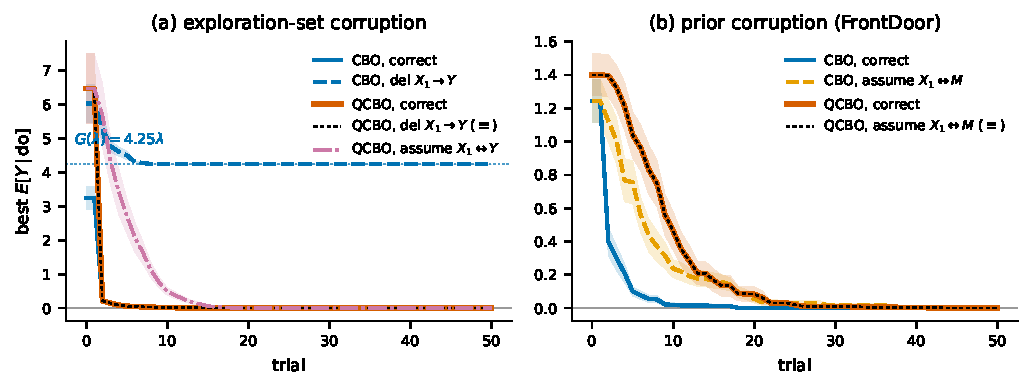
\includegraphics[width=\textwidth]{figures/minimal_misspec}
  \caption{Correct and misspecified trajectories, mean $\pm$ standard error
  over $30$ seeds. Left: a wrong fine graph removes the optimal arm, while
  QCBO is unchanged for a quotient-invisible edit. Right: prior corruption
  slows fine CBO transiently, while QCBO remains exactly invariant.}
  \label{fig:minimal-misspec}
\end{figure*}

\subsection{Action-space price and refinement}
\label{sec:exp-c}

The \textsc{MediatedChain} graph in Appendix~\ref{app:dags} has
$X_1\to X_2\to Y$, with $X_2=2X_1+\varepsilon_2$ and
$Y=(X_2-4)^2+\varepsilon_Y$. The fine arm $\doo(X_1=2)$ leaves $X_2$
free to respond naturally around $4$ and attains
$y^\star=\operatorname{Var}(\varepsilon_2)=0.04$. In contrast, fixed QCBO
has only the whole-cluster arm $\{X_1,X_2\}$. This arm must clamp $X_2$
inside its intervention domain $[-2,2]$; once $X_2$ is clamped, $X_1$ has
no remaining effect on $Y$. The best allowed choice is therefore $X_2=2$,
which yields
\[
 V(\Pi)=4,
 \qquad y^\star=0.04,
 \qquad \Delta(\Pi)=3.96.
\]
Consequently, every fixed-QCBO incumbent has instantaneous regret at least
$3.96$, and Proposition~\ref{prop:floor} gives the permanent lower bound
$R_T\ge3.96T$. Fine CBO does not incur this floor because its MIS retains
$\{X_1\}$. HQCBO removes it only after the declared hierarchy splits
$\{X_1,X_2\}$ and exposes the singleton arm. Figure~\ref{fig:minimal-refine}
shows the resulting best-value and cumulative-regret trajectories. CBO,
fixed QCBO, and HQCBO finish at $0.0400\pm0.0000$,
$4.0000\pm0.0000$, and $0.0400\pm0.0000$, with cumulative regrets
$5.46\pm1.61$, $243.23\pm0.90$, and $36.97\pm1.18$,
respectively. HQCBO refines at trial $7.4\pm0.1$; all $30$ declared splits
are accepted. The fixed-QCBO result exceeds the theoretical floor
$60\times3.96=237.6$ only by its within-space optimization error. The
experiment demonstrates recovery for this declared split; it does not imply
that the plateau rule always selects a useful refinement.

\begin{figure}[t]
  \centering
  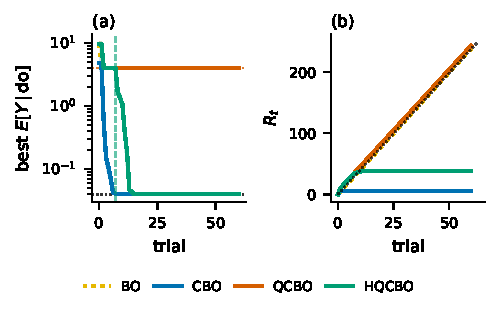
\includegraphics[width=\linewidth]{figures/minimal_refine}
  \caption{\textsc{MediatedChain} over $30$ seeds. Top: mean $\pm$
  standard error best-so-far population value and mean refinement time.
  Bottom: mean cumulative incumbent regret, excluding the shared initial
  incumbent. Fixed QCBO cannot execute $\doo(X_1)$; refinement exposes it.}
  \label{fig:minimal-refine}
\end{figure}

\subsection{Portability across optimizer families}
\label{sec:exp-d}

Figure~\ref{fig:family-suite} compares each quotient construction with its
base optimizer on the eight tasks described above; all corresponding DAGs
and C-DAGs are in Appendix~\ref{app:dags}. The structural prediction is
exact: QDCBO is invariant in all $60$ paired dynamic runs and QMCBO in all
$40$ paired model-based runs, whereas their base methods change under the
same graph-view perturbations. This confirms that the quotient contract is
independent of the family-specific acquisition and surrogate construction.

Finite-budget performance is deliberately reported separately from
invariance. Table~\ref{tab:family-effects} gives the final population value
and paired quotient disadvantage for each task. For $\downarrow$ rows the
paired difference is quotient minus base; for $\uparrow$ rows it is base
minus quotient. Positive values therefore always mean that the quotient
ended worse. These are finite-budget effects incorporating optimization and
initialization, not estimates of the theoretical action-space quantity
$\Delta(\Pi)$.

\begin{figure*}[t]
  \centering
  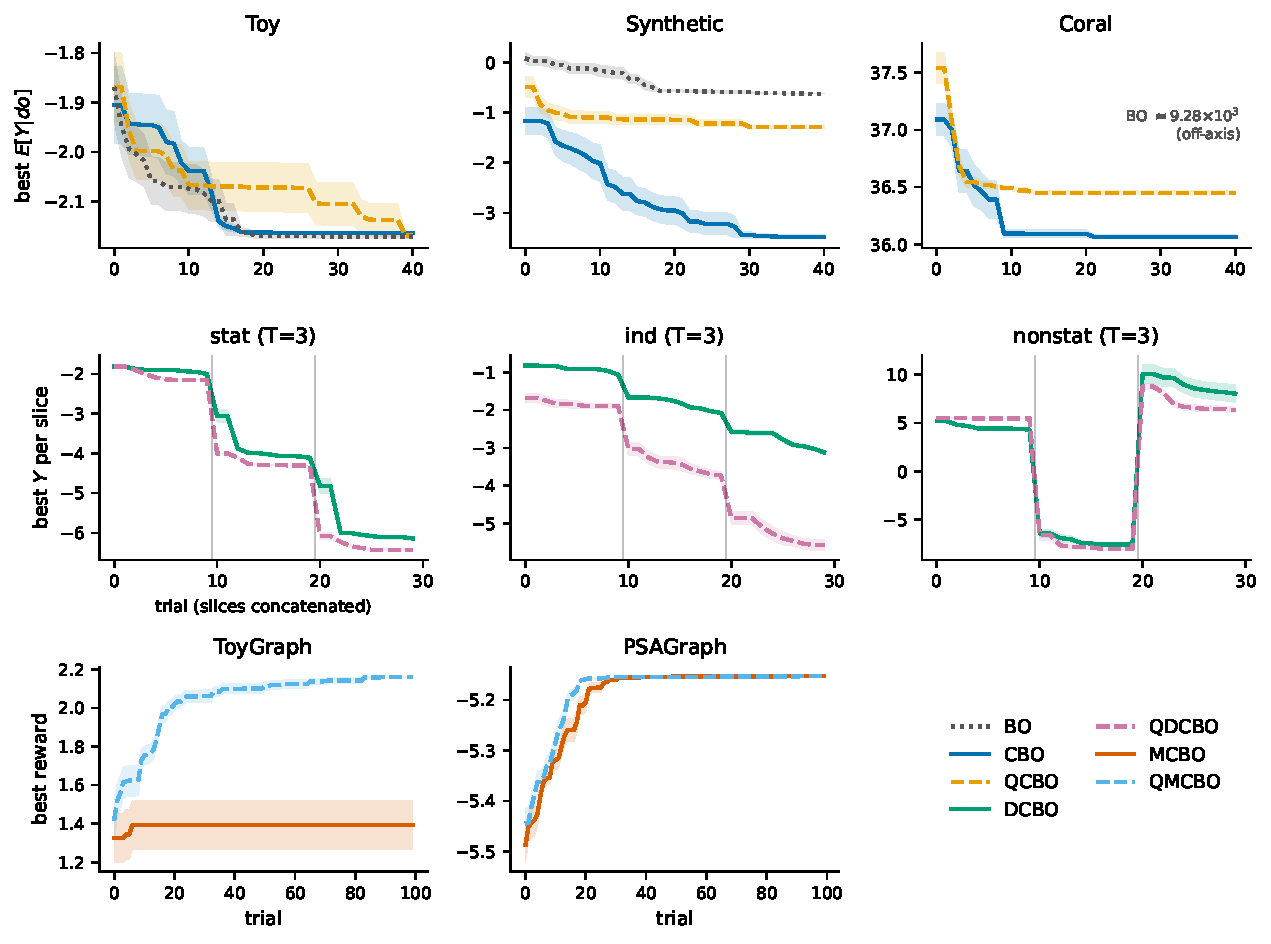
\includegraphics[width=\textwidth]{figures/family_suite}
  \caption{Quotient methods and their bases under the released family
  protocols, mean $\pm$ standard error. Top: CBO minimization. Middle:
  dynamic minimization over three time slices. Bottom: MCBO maximization.}
  \label{fig:family-suite}
\end{figure*}

\begin{table*}[t]
  \centering
  \caption{Final population values and paired quotient disadvantage. Each
  task label carries its optimization direction. Positive paired effects
  mean worse quotient performance; intervals are paired-$t$ $95\%$ CIs.}
  \label{tab:family-effects}
  \small
  \adjustbox{max width=\textwidth}{% Auto-generated by scripts/emit_paired_effects.py -- do not edit.
\begin{tabular}{@{}lccc@{}}
\toprule
\textbf{Task} & \textbf{Base} & \textbf{Quotient} & $\boldsymbol{\Delta}$ \textbf{[95\% CI]} \\
\midrule
\multicolumn{4}{@{}l}{\emph{\CBO{} vs \QCBO{} ($n{=}10$)}} \\
Toy $\downarrow$ & $-2.16{\scriptstyle\,\pm\,}0.00$ & $-2.17{\scriptstyle\,\pm\,}0.01$ & $0.00$ $[-0.02,\,+0.01]$ \\
Synthetic $\downarrow$ & $-3.57{\scriptstyle\,\pm\,}0.00$ & $-1.31{\scriptstyle\,\pm\,}0.00$ & $+2.25$ $[+2.25,\,+2.26]$ \\
Coral $\downarrow$ & $36.04{\scriptstyle\,\pm\,}0.01$ & $36.40{\scriptstyle\,\pm\,}0.01$ & $+0.36$ $[+0.32,\,+0.39]$ \\
\addlinespace[2pt]
\multicolumn{4}{@{}l}{\emph{DCBO vs \QDCBO{} ($n{=}20$)}} \\
Stationary $\downarrow$ & $-6.12{\scriptstyle\,\pm\,}0.05$ & $-6.40{\scriptstyle\,\pm\,}0.03$ & $-0.27$ $[-0.39,\,-0.15]$ \\
Independent $\downarrow$ & $-3.13{\scriptstyle\,\pm\,}0.06$ & $-5.55{\scriptstyle\,\pm\,}0.13$ & $-2.43$ $[-2.69,\,-2.17]$ \\
Nonstationary $\downarrow$ & $7.01{\scriptstyle\,\pm\,}0.83$ & $5.78{\scriptstyle\,\pm\,}0.02$ & $-1.23$ $[-2.98,\,+0.52]$ \\
\addlinespace[2pt]
\multicolumn{4}{@{}l}{\emph{MCBO vs \QMCBO{} ($n{=}20$)}} \\
ToyGraph $\uparrow$ & $1.39{\scriptstyle\,\pm\,}0.13$ & $2.16{\scriptstyle\,\pm\,}0.00$ & $-0.77$ $[-1.04,\,-0.50]$ \\
PSAGraph $\uparrow$ & $-5.15{\scriptstyle\,\pm\,}0.00$ & $-5.15{\scriptstyle\,\pm\,}0.00$ & $\approx 0$ \\
\bottomrule
\end{tabular}
}
\end{table*}

\clearpage

\section{Related work}
\label{sec:related}

Graph-agnostic and causal entropy optimization methods learn over candidate
graphs online
\citep{mukherjeeGraphAgnosticCausal2024,branchiniCausalEntropyOptimization2023},
while causal-bandit guarantees price learning an unknown graph within the
horizon \citep{luCausalBanditsUnknown2021}. Our setting instead studies
commitment to a fixed coarse input. These approaches are complementary: a
graph learner could operate over, or trigger refinement of, a quotient.

The construction builds on cluster-DAG identification
\citep{CausalEffectIdentification} and is related to causal abstraction and
macro-level structure learning
\citep{beckersAbstractingCausalModels2019,madaleno2026a}. We coarsen
manipulable inputs and explicitly characterize the actions removed by that
choice.

\section{Limitations}
\label{sec:limitations}

Exact invariance requires the correct quotient; quotient-visible errors and
incorrect partitions remain harmful. The zero-price condition is sufficient
and structural, and its cross-world consequence is not directly testable
from single-world data. Refinement is heuristic, with recovery conditional
on visiting a lossless partition and on consistency of the base optimizer.
Different partitions also induce different arm counts, initialization costs,
and intervention costs. Finally, QMCBO inherits the causal-sufficiency
assumption of its model-based factorization.

\section{Conclusion}
\label{sec:conclusion}

Coarsening makes precisely those graph distinctions that disappear in the
quotient irrelevant to optimization. Within the resulting protected class,
the complete trajectory is invariant. The price is the optimal value of
fine interventions excluded by the partition, which is monotone under
refinement and zero under the stated structural conditions. Theoretical and
empirical results show that quotienting can prevent catastrophic graph
errors, while hierarchical refinement provides a conditional route back to
the fine action space.

\bibliographystyle{abbrvnat}
\bibliography{references}

\appendix
\onecolumn
\raggedbottom

\section{Proofs and additional technical results}
\label{app:proofs}

\subsection{Minimal intervention sets and quotient values}

\begin{lemma}[MIS reduction]
\label{lem:mis-reduction}
Let $G$ be an ADMG with manipulable vertices $M$ and target $Y$. For
$\emptyset\ne W\subseteq M$, let
$W'=W\cap\An(Y)$ in $G_{\bar W}$. Then
\begin{enumerate}[label=(\roman*),leftmargin=1.6em,itemsep=1pt]
\item $P(Y\mid\doo(W=w))=P(Y\mid\doo(W'=w|_{W'}))$;
\item $W'$ is a MIS, or is empty if no member reaches $Y$; and
\item restricting the action search to $\mathrm{MIS}(G)$ does not change
the minimum population value.
\end{enumerate}
\end{lemma}

\begin{proof}
In $G_{\bar W}$, variables in $W\setminus W'$ have no directed path to
$Y$, so dropping them from the intervention does not change the distribution
of $Y$. Every directed path from a member of $W'$ to $Y$ avoids all
intervened vertices and remains after the edges into $W\setminus W'$ are
restored; hence $W'$ satisfies the MIS condition. Applying this reduction to
every candidate intervention proves the equality of minima.
\end{proof}

Consequently, the best value over the quotient MIS expanded to fine
variables equals $V(\Pi)$ in Equation~\eqref{eq:price}.

\subsection{Proofs of the main structural results}

\begin{proof}[Proof of Proposition~\ref{prop:contract}]
Write the run as decisions $d_1,d_2,\ldots$ and datasets
$\mathcal D_0,\mathcal D_1,\ldots$, with
\[
d_t=f_t\!\left(Q_\Pi(H),\mathcal D_{t-1},\omega_t,\eta\right).
\]
Equal quotients, initial data, random streams, and hyperparameters imply
equal first decisions. The fixed true SCM produces the same coupled
observation, so the updated datasets also agree. Induction gives equality of
every decision, observation, incumbent, and stopping event.
\end{proof}

\begin{proof}[Proof of Proposition~\ref{prop:price}]
Every union of clusters in $\Pi$ is a union of clusters in a refinement
$\Pi'$, and every such union is available at the singleton partition. The
three population minima are therefore taken over nested action families:
$V(\Pi_\bot)\le V(\Pi')\le V(\Pi)$. Equality between the first and last
terms holds exactly when a global fine optimum belongs to
$\mathcal U(\Pi)$.
\end{proof}

\begin{proof}[Proof of Proposition~\ref{prop:free}]
Fix $A$ and $a$. Consistency and cross-world independence give
\[
\begin{aligned}
 \E[Y_a]
 &=\int \E[Y_{a,b}\mid B_a=b],dP(B_a=b)\\
 &=\int \E[Y_{a,b}],dP(B_a=b)\\
 &\ge \inf_{b\in D_B(a)}\E[Y_{a,b}],
\end{aligned}
\]
where support inclusion justifies the final inequality. Thus the whole
cluster closure can match or improve every fine intervention:
$\mu^\star(\operatorname{cl}_\Pi(A))\le\mu^\star(A)$. Taking minima and
using $\mathcal U(\Pi)\subseteq\mathcal U(\Pi_\bot)$ gives equality.
\end{proof}

\begin{lemma}[Cluster containment implies cross-world independence]
\label{lem:ccc}
Under the model in Definition~\ref{def:ccc}, cluster-contained confounding
implies $B_a\perp Y_{a,b}$ for every $A$, $a$, and $b\in D_B(a)$.
\end{lemma}

\begin{proof}
After $\doo(A=a)$, recursive substitution expresses $B_a$ as a measurable
function of $\mathbf U_B(A)$. After clamping the entire cluster closure, it
expresses $Y_{a,b}$ as a measurable function of $\mathbf U_Y(A)$. The two
exogenous ancestor sets are disjoint by Definition~\ref{def:ccc} and the
exogenous variables are mutually independent, so the two functions are
independent. Full intervention support separately implies
$\operatorname{supp}(B_a)\subseteq D_B(a)$, proving
Corollary~\ref{cor:zero-price}.
\end{proof}

\begin{proof}[Proof of Theorem~\ref{thm:separation}]
For part (i), use \textsc{ParallelParent} with manipulable variables
$\{X_1,X_2\}$, domains $[-3,3]^2$, edges $X_1\to Y$ and $X_2\to Y$,
latent $X_1\leftrightarrow X_2$, and partition
$\{\{X_1,X_2\},\{Y\}\}$. Choose the objective curvature so that the
best $\{X_2\}$-only intervention has value $\beta$, while the joint arm
attains $y^\star=0$. Deleting $X_1\to Y$ preserves the quotient through
$X_2\to Y$ but leaves $\mathrm{MIS}(H)=\{\{X_2\}\}$. Every executed
intervention and every eligible incumbent therefore has regret at least
$\beta$, giving $R_T\ge\beta T$. The whole-cluster arm remains globally
optimal, so $\Delta(\Pi)=0$.

For part (ii), Proposition~\ref{prop:contract} makes the trajectory and
regret constant over $E_\Pi(\Gg)$. Adding and subtracting $V(\Pi)$ in each
regret term gives
\[
 r_t=\Delta(\Pi)+\mu(\hat a_t)-V(\Pi).
\]
The second term is nonnegative because every incumbent is an executed
cluster-union action. Summing over $t$ yields the stated decomposition.
\end{proof}

\begin{proof}[Proof of Proposition~\ref{prop:floor}]
Every incumbent belongs to the fixed action family, hence
$\mu(\hat a_t)\ge V(\Pi)$. Subtracting
$y^\star=V(\Pi_\bot)$ gives $r_t\ge\Delta(\Pi)$; summation gives the
cumulative bound.
\end{proof}

\begin{proof}[Proof of Corollary~\ref{cor:recovery}]
At a visited lossless partition, incumbent consistency gives
$\mu(\hat a_t)\to V(\Pi_J)=y^\star$, hence $r_t\to0$ almost surely.
Ces\`aro averaging then gives $R_T/T\to0$.
\end{proof}

\begin{proof}[Proof of Corollary~\ref{cor:adaptive-invariance}]
Proceed by induction over refinement phases. Within phase $j$, all
graph-dependent behavior factors through $(\Pi_j,\Gg^{\Pi_j})$. Equal
quotients and equal trajectory prefixes therefore produce the same phase
trajectory, plateau decision, and next split. Repeating this argument through
$\Pi_J$ proves equality of the adaptive trajectories.
\end{proof}

\subsection{Necessity, refinement validity, and model-based soundness}

\begin{proposition}[Necessity of the quotient contract]
\label{prop:converse}
If, for every ADMG $\Gg$, the trajectory map is constant on
$E_\Pi(\Gg)$ at fixed $(\mathcal D,\omega,\eta)$, then the trajectory map
factors through $Q_\Pi$.
\end{proposition}

\begin{proof}
Constancy on every fiber of $Q_\Pi$ makes
$\bar\tau(q):=\tau(H)$ well defined for any $H$ satisfying
$Q_\Pi(H)=q$. Hence $\tau=\bar\tau\circ Q_\Pi$.
\end{proof}

\begin{proposition}[Refinement can invalidate a quotient]
\label{prop:refinement-validity}
There exist a valid partition $\Pi$ and a refinement $\Pi'\preceq\Pi$ for
which $\Gg^\Pi$ is acyclic but $\Gg^{\Pi'}$ contains a directed cycle.
Validity must therefore be checked after every split.
\end{proposition}

\begin{proof}
Let the fine graph contain $a_1\to b_1$ and $b_2\to a_2$. The single
cluster $\{a_1,a_2,b_1,b_2\}$ has an acyclic one-node quotient. Refining
it into $\{a_1,a_2\}$ and $\{b_1,b_2\}$ exposes both quotient directions
and produces a two-cycle.
\end{proof}

\begin{proposition}[Soundness of joint cluster mechanisms]
\label{prop:cluster-soundness}
Under causal sufficiency and a valid partition, every intervention on a
union of clusters $S$ satisfies
\[
 P(\mathbf V\mid\doo(\mathbf x_S))
 =\prod_{C\notin S}
 P(\mathbf X_C\mid\mathbf X_{\mathrm{pa}(C)})
 \big|_{\mathbf X_S=\mathbf x_S}.
\]
\end{proposition}

\begin{proof}
Apply the fine truncated factorization and group its factors by clusters.
Within each cluster, the chain rule combines the member-wise factors into
the joint conditional mechanism. Validity orders these mechanisms along the
quotient DAG. The joint conditional is essential: replacing it by the
product of member-wise marginals would discard within-cluster dependence.
\end{proof}

\begin{proposition}[Sub-cluster effects are not identified by cluster mechanisms]
\label{prop:qexposure}
There exist two causally sufficient SCMs with the same valid quotient, joint
cluster mechanisms, and whole-cluster interventional distributions, but
different values of $P(Y\mid\doo(A=a))$ for a strict subset $A$ of a
cluster.
\end{proposition}

\begin{proof}
Let $C=\{X_2,X_3\}$ be a root cluster and $Y=X_2+\varepsilon_Y$. In one
SCM take $X_2=\varepsilon_2$ and $X_3=aX_2+\varepsilon_3$; in another,
choose the reverse linear-Gaussian factorization of the same joint
distribution. The two models agree on the joint law of $C$ and on every
whole-cluster intervention. Under $\doo(X_3=x)$, however, $X_2$ remains
mean zero in the first model and changes linearly with $x$ in the second.
Thus quotient-respecting inputs do not identify the sub-cluster effect.
\end{proof}

\clearpage
\section{Identification and numerical estimation}
\label{app:estimators}

The complete identification check is performed on the ADMG supplied to the
optimizer. When the query is identified, the returned functional is
instantiated by a sound library of GP plug-in estimators. For a valid
backdoor set $Z$, the estimator is Equation~\eqref{eq:backdoor-prior}. For a
frontdoor mediator $M$ between treatment $X$ and target $Y$, it uses
\begin{equation}
 \widehat p(y\mid\doo(x))=
 \int \widehat p(m\mid x)
 \left\{\int \widehat p(y\mid m,x')\,\mathrm d\widehat P(x')\right\}
 \mathrm dm.
 \label{eq:frontdoor-estimator}
\end{equation}
Under causal sufficiency it instead evaluates the truncated factorization
in Equation~\eqref{eq:g-formula}. Required conditional means and densities
are fitted from the observational sample with GP regressions and integrated
numerically over the intervention domain. If complete identification fails,
or if the identified functional lies outside this sound implementation
library, the arm receives the common uninformative prior
$m_A(a)=\bar Y_{\mathrm{obs}}$. Interventional observations subsequently
update the arm's GP in the usual way.

This distinction is important: complete identification determines whether a
causal effect is a functional of the observational law, whereas backdoor,
frontdoor, and $g$-computation describe the particular functionals currently
implemented. The latter list is deliberately not presented as complete for
arbitrary ADMGs.

\section{Experimental details}
\label{app:additional-results}

\paragraph{Controlled suite.}
All methods receive the same sampled observational dataset and exact
population intervention evaluator. Initial intervention values are sampled
uniformly from the declared domains and their outcomes are computed by the
same closed-form evaluator used during sequential optimization. Each run
logs the selected arm and intervention values in addition to the incumbent.
For protected perturbations, arm sequences and intervention values are
compared exactly and incumbent values to $10^{-8}$, allowing for numerical
GP optimization. The complete perturbation taxonomy is reported in
Table~\ref{tab:minimal-taxonomy}.

\begin{table}[H]
  \centering
  \caption{Controlled misspecifications and measured paired trajectory
  deviations. Rows whose quotient is unchanged are predicted invariant by
  Proposition~\ref{prop:contract}.}
  \label{tab:minimal-taxonomy}
  \small
  \adjustbox{max width=\textwidth}{\begin{tabular}{llcccc}
\hline
Condition & Edit & Quotient & Fine MIS & Fine prior & Role\\
 & & changed & changed & changed & \\
\hline
A1 (PP) & delete $X_1\to Y$ & no & yes & -- & primary\\
A2 (PP) & add $X_1\to X_2$ & no & no & yes & diagnostic\\
A3 (PP) & add $X_1\leftrightarrow Y$ & yes & no & yes & diagnostic\\
B1 (FD) & add $X_1\leftrightarrow M$ & no & no & yes & primary\\
\hline
\end{tabular}
}
\end{table}

\paragraph{Family suite.}
The CBO/QCBO comparison uses a common arm-based implementation with
cost-normalized EI. DCBO/QDCBO and MCBO/QMCBO retain the released base
implementations, including their acquisition and update schedules. Thus the
portability experiment tests whether quotient invariance survives these
family-specific choices rather than forcing every method through one
optimizer. All plots show means and standard errors over paired seeds. The
paired intervals in Table~\ref{tab:family-effects} use the seedwise
differences defined in Section~\ref{sec:exp-design}.

\section{Dataset graphs and their quotients}
\label{app:dags}

For every distinct dataset topology, the following figures show the fine
graph with its coarse partition and the quotient graph consumed by the
optimizer. Manipulable variables are orange, targets are blue, dash-dotted
edges denote latent confounding, and dashed boxes indicate manipulable
clusters. Graph-isomorphic benchmark pairs are shown once under their shared
topology.

\begingroup
\let\savedfigure\figure
\let\endsavedfigure\endfigure
\renewenvironment{figure}[1][]{\savedfigure[H]}{\endsavedfigure}
% Auto-generated by scripts/emit_dataset_tikz.py -- do not edit by hand.

\begin{figure}[t]\centering
\adjustbox{max width=0.58\linewidth,valign=c}{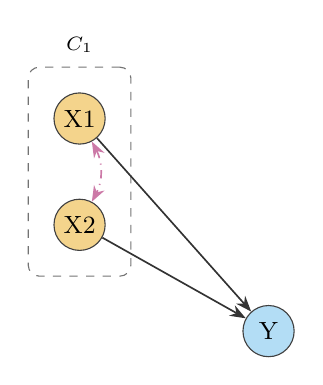
\begin{tikzpicture}
  \node[mannode] (nX1) at (0.00,0.00) {X1};
  \node[mannode] (nX2) at (0.00,-1.35) {X2};
  \node[tgtnode] (nY) at (2.40,-2.70) {Y};
  \draw[diredge] (nX1) -- (nY);
  \draw[diredge] (nX2) -- (nY);
  \draw[biintra] (nX1) to[bend left=28] (nX2);
  \begin{scope}[on background layer]
    \node[clbox,fit=(nX1)(nX2),label={[label distance=0.5mm]above:{\scriptsize$C_{1}$}}] {};
  \end{scope}
\end{tikzpicture}}\hfill
\adjustbox{max width=0.38\linewidth,valign=c}{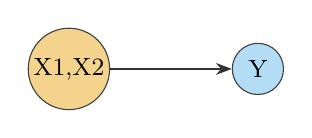
\begin{tikzpicture}
  \node[tgtnode] (nY) at (2.40,0.00) {Y};
  \node[mannode] (nX1X2) at (0.00,0.00) {X1,X2};
  \draw[diredge] (nX1X2) -- (nY);
\end{tikzpicture}}
\caption{\textbf{ParallelParent (MinimalBench, Exp.\ A).} Fine DAG with coarse partition (left) and quotient C-DAG (right), in the convention of Fig.~\ref{fig:motivating}: manipulable variables orange, target blue, dash-dotted latent confounding; dashed boxes are the manipulable clusters. The intra-cluster $X_1\leftrightarrow X_2$ disappears in the quotient; deleting $X_1\to Y$ leaves $C_1\to Y$ alive through $X_2\to Y$ (quotient-redundant).}
\label{fig:dag-parallelparent}
\end{figure}

\begin{figure}[t]\centering
\adjustbox{max width=0.58\linewidth,valign=c}{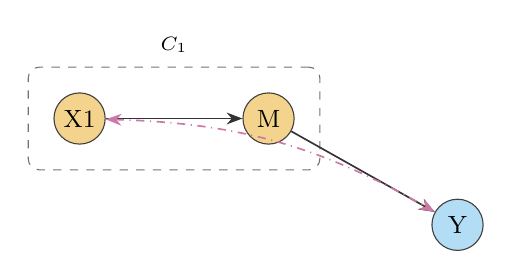
\begin{tikzpicture}
  \node[mannode] (nX1) at (0.00,0.00) {X1};
  \node[mannode] (nM) at (2.40,0.00) {M};
  \node[tgtnode] (nY) at (4.80,-1.35) {Y};
  \draw[diredge] (nX1) -- (nM);
  \draw[diredge] (nM) -- (nY);
  \draw[bicross] (nX1) to[bend left=14] (nY);
  \begin{scope}[on background layer]
    \node[clbox,fit=(nX1)(nM),label={[label distance=0.5mm]above:{\scriptsize$C_{1}$}}] {};
  \end{scope}
\end{tikzpicture}}\hfill
\adjustbox{max width=0.38\linewidth,valign=c}{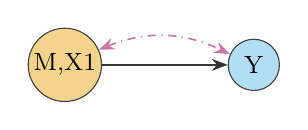
\begin{tikzpicture}
  \node[mannode] (nMX1) at (0.00,0.00) {M,X1};
  \node[tgtnode] (nY) at (2.40,0.00) {Y};
  \draw[diredge] (nMX1) -- (nY);
  \draw[bicross] (nMX1) to[bend left=24] (nY);
\end{tikzpicture}}
\caption{\textbf{FrontDoor (MinimalBench, Exp.\ B).} Fine DAG with coarse partition (left) and quotient C-DAG (right), in the convention of Fig.~\ref{fig:motivating}: manipulable variables orange, target blue, dash-dotted latent confounding; dashed boxes are the manipulable clusters. The quotient is a bow ($C_1\to Y$, $C_1\leftrightarrow Y$): the cluster arm runs on the uninformative prior tier in every condition, so the assumed intra-cluster $X_1\leftrightarrow M$ cannot change it.}
\label{fig:dag-frontdoor}
\end{figure}

\begin{figure}[t]\centering
\adjustbox{max width=0.58\linewidth,valign=c}{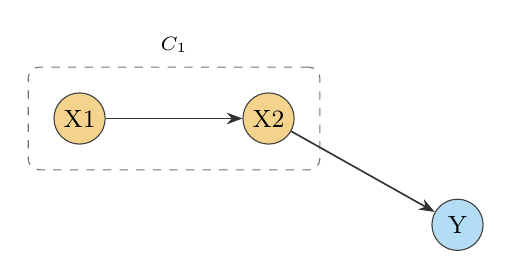
\begin{tikzpicture}
  \node[mannode] (nX1) at (0.00,0.00) {X1};
  \node[mannode] (nX2) at (2.40,0.00) {X2};
  \node[tgtnode] (nY) at (4.80,-1.35) {Y};
  \draw[diredge] (nX1) -- (nX2);
  \draw[diredge] (nX2) -- (nY);
  \begin{scope}[on background layer]
    \node[clbox,fit=(nX1)(nX2),label={[label distance=0.5mm]above:{\scriptsize$C_{1}$}}] {};
  \end{scope}
\end{tikzpicture}}\hfill
\adjustbox{max width=0.38\linewidth,valign=c}{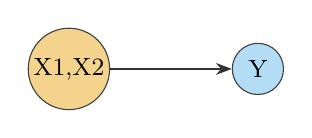
\begin{tikzpicture}
  \node[tgtnode] (nY) at (2.40,0.00) {Y};
  \node[mannode] (nX1X2) at (0.00,0.00) {X1,X2};
  \draw[diredge] (nX1X2) -- (nY);
\end{tikzpicture}}
\caption{\textbf{MediatedChain (MinimalBench, Exp.\ C).} Fine DAG with coarse partition (left) and quotient C-DAG (right), in the convention of Fig.~\ref{fig:motivating}: manipulable variables orange, target blue, dash-dotted latent confounding; dashed boxes are the manipulable clusters. The policy box restricts $D(X_2)$ to $[-2,2]$; the fine optimum $\doo(X_1{=}2)$ drives $X_2$ to $4$, outside the box.}
\label{fig:dag-mediatedchain}
\end{figure}

\begin{figure}[t]\centering
\adjustbox{max width=0.58\linewidth,valign=c}{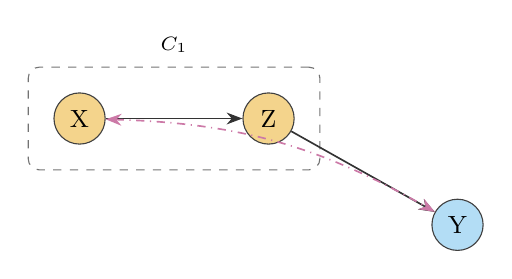
\begin{tikzpicture}
  \node[mannode] (nX) at (0.00,0.00) {X};
  \node[mannode] (nZ) at (2.40,0.00) {Z};
  \node[tgtnode] (nY) at (4.80,-1.35) {Y};
  \draw[diredge] (nX) -- (nZ);
  \draw[diredge] (nZ) -- (nY);
  \draw[bicross] (nX) to[bend left=14] (nY);
  \begin{scope}[on background layer]
    \node[clbox,fit=(nX)(nZ),label={[label distance=0.5mm]above:{\scriptsize$C_{1}$}}] {};
  \end{scope}
\end{tikzpicture}}\hfill
\adjustbox{max width=0.38\linewidth,valign=c}{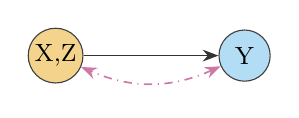
\begin{tikzpicture}
  \node[tgtnode] (nY) at (2.40,0.00) {Y};
  \node[mannode] (nXZ) at (0.00,0.00) {X,Z};
  \draw[diredge] (nXZ) -- (nY);
  \draw[bicross] (nY) to[bend left=24] (nXZ);
\end{tikzpicture}}
\caption{\textbf{ToyGraph (CBO family).} Fine DAG with coarse partition (left) and quotient C-DAG (right), in the convention of Fig.~\ref{fig:motivating}: manipulable variables orange, target blue, dash-dotted latent confounding; dashed boxes are the manipulable clusters. The quotient is a bow ($C_1\to Y$, $C_1\leftrightarrow Y$): $\doo(C_1)$ is not identifiable from the C-DAG, so the arm runs on the uninformative prior tier.}
\label{fig:dag-toy}
\end{figure}

\begin{figure}[t]\centering
\adjustbox{max width=0.58\linewidth,valign=c}{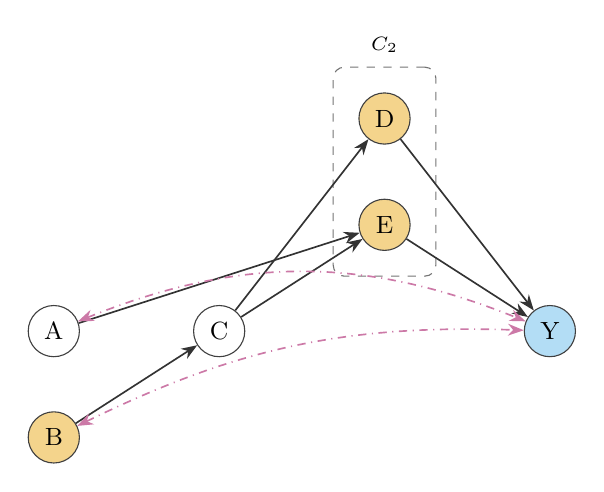
\begin{tikzpicture}
  \node[obsnode] (nA) at (0.00,-2.70) {A};
  \node[mannode] (nB) at (0.00,-4.05) {B};
  \node[obsnode] (nC) at (2.10,-2.70) {C};
  \node[mannode] (nD) at (4.20,0.00) {D};
  \node[mannode] (nE) at (4.20,-1.35) {E};
  \node[tgtnode] (nY) at (6.30,-2.70) {Y};
  \draw[diredge] (nB) -- (nC);
  \draw[diredge] (nC) -- (nD);
  \draw[diredge] (nA) -- (nE);
  \draw[diredge] (nC) -- (nE);
  \draw[diredge] (nD) -- (nY);
  \draw[diredge] (nE) -- (nY);
  \draw[bicross] (nB) to[bend left=14] (nY);
  \draw[bicross] (nA) to[bend left=22] (nY);
  \begin{scope}[on background layer]
    \node[clbox,fit=(nD)(nE),label={[label distance=0.5mm]above:{\scriptsize$C_{2}$}}] {};
  \end{scope}
\end{tikzpicture}}\hfill
\adjustbox{max width=0.38\linewidth,valign=c}{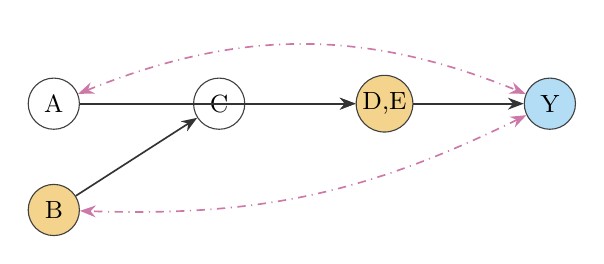
\begin{tikzpicture}
  \node[mannode] (nB) at (0.00,-1.35) {B};
  \node[obsnode] (nC) at (2.10,0.00) {C};
  \node[obsnode] (nA) at (0.00,0.00) {A};
  \node[mannode] (nDE) at (4.20,0.00) {D,E};
  \node[tgtnode] (nY) at (6.30,0.00) {Y};
  \draw[diredge] (nC) -- (nDE);
  \draw[diredge] (nB) -- (nC);
  \draw[diredge] (nA) -- (nDE);
  \draw[diredge] (nDE) -- (nY);
  \draw[bicross] (nY) to[bend left=14] (nB);
  \draw[bicross] (nA) to[bend left=22] (nY);
\end{tikzpicture}}
\caption{\textbf{CompleteGraph (CBO family).} Fine DAG with coarse partition (left) and quotient C-DAG (right), in the convention of Fig.~\ref{fig:motivating}: manipulable variables orange, target blue, dash-dotted latent confounding; dashed boxes are the manipulable clusters.}
\label{fig:dag-complete}
\end{figure}

\begin{figure}[t]\centering
\adjustbox{max width=0.58\linewidth,valign=c}{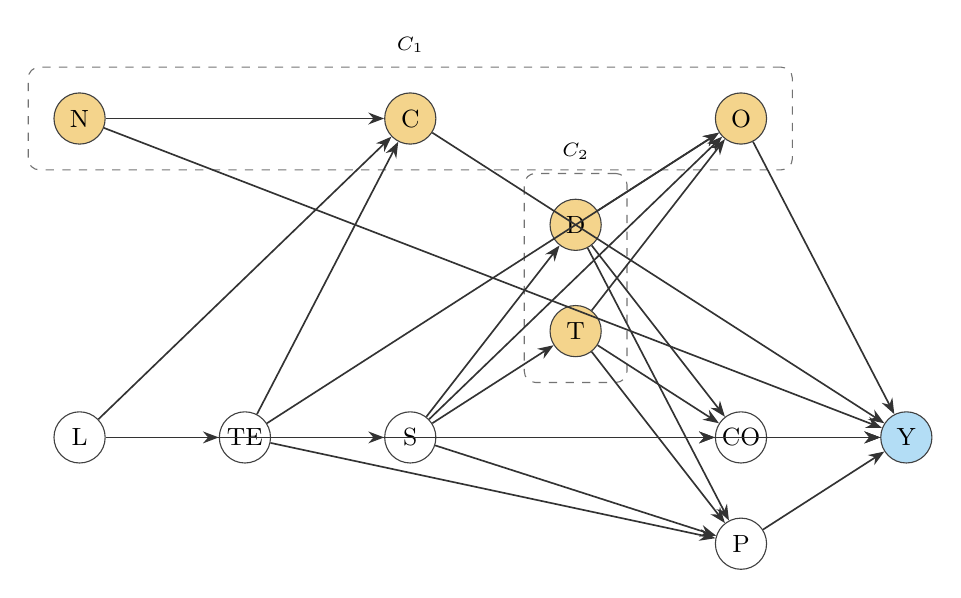
\begin{tikzpicture}
  \node[mannode] (nN) at (0.00,0.00) {N};
  \node[obsnode] (nL) at (0.00,-4.05) {L};
  \node[obsnode] (nTE) at (2.10,-4.05) {TE};
  \node[mannode] (nC) at (4.20,0.00) {C};
  \node[obsnode] (nS) at (4.20,-4.05) {S};
  \node[mannode] (nT) at (6.30,-2.70) {T};
  \node[mannode] (nD) at (6.30,-1.35) {D};
  \node[obsnode] (nP) at (8.40,-5.40) {P};
  \node[mannode] (nO) at (8.40,0.00) {O};
  \node[obsnode] (nCO) at (8.40,-4.05) {CO};
  \node[tgtnode] (nY) at (10.50,-4.05) {Y};
  \draw[diredge] (nL) -- (nTE);
  \draw[diredge] (nL) -- (nC);
  \draw[diredge] (nL) -- (nY);
  \draw[diredge] (nN) -- (nC);
  \draw[diredge] (nN) -- (nY);
  \draw[diredge] (nTE) -- (nC);
  \draw[diredge] (nTE) -- (nS);
  \draw[diredge] (nTE) -- (nP);
  \draw[diredge] (nTE) -- (nO);
  \draw[diredge] (nTE) -- (nCO);
  \draw[diredge] (nTE) -- (nY);
  \draw[diredge] (nS) -- (nT);
  \draw[diredge] (nS) -- (nD);
  \draw[diredge] (nS) -- (nP);
  \draw[diredge] (nS) -- (nO);
  \draw[diredge] (nS) -- (nCO);
  \draw[diredge] (nT) -- (nP);
  \draw[diredge] (nT) -- (nO);
  \draw[diredge] (nT) -- (nCO);
  \draw[diredge] (nD) -- (nP);
  \draw[diredge] (nD) -- (nO);
  \draw[diredge] (nD) -- (nCO);
  \draw[diredge] (nP) -- (nY);
  \draw[diredge] (nO) -- (nY);
  \draw[diredge] (nC) -- (nY);
  \draw[diredge] (nCO) -- (nY);
  \begin{scope}[on background layer]
    \node[clbox,fit=(nC)(nN)(nO),label={[label distance=0.5mm]above:{\scriptsize$C_{1}$}}] {};
  \end{scope}
  \begin{scope}[on background layer]
    \node[clbox,fit=(nD)(nT),label={[label distance=0.5mm]above:{\scriptsize$C_{2}$}}] {};
  \end{scope}
\end{tikzpicture}}\hfill
\adjustbox{max width=0.38\linewidth,valign=c}{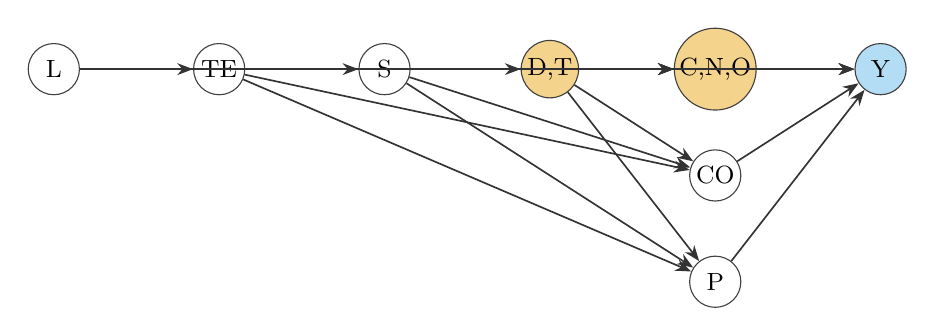
\begin{tikzpicture}
  \node[mannode] (nDT) at (6.30,0.00) {D,T};
  \node[obsnode] (nTE) at (2.10,0.00) {TE};
  \node[mannode] (nCNO) at (8.40,0.00) {C,N,O};
  \node[obsnode] (nS) at (4.20,0.00) {S};
  \node[obsnode] (nCO) at (8.40,-1.35) {CO};
  \node[obsnode] (nP) at (8.40,-2.70) {P};
  \node[obsnode] (nL) at (0.00,0.00) {L};
  \node[tgtnode] (nY) at (10.50,0.00) {Y};
  \draw[diredge] (nL) -- (nY);
  \draw[diredge] (nS) -- (nCNO);
  \draw[diredge] (nCNO) -- (nY);
  \draw[diredge] (nTE) -- (nCNO);
  \draw[diredge] (nTE) -- (nP);
  \draw[diredge] (nDT) -- (nCNO);
  \draw[diredge] (nS) -- (nCO);
  \draw[diredge] (nL) -- (nTE);
  \draw[diredge] (nP) -- (nY);
  \draw[diredge] (nDT) -- (nCO);
  \draw[diredge] (nTE) -- (nCO);
  \draw[diredge] (nDT) -- (nP);
  \draw[diredge] (nL) -- (nCNO);
  \draw[diredge] (nS) -- (nP);
  \draw[diredge] (nCO) -- (nY);
  \draw[diredge] (nS) -- (nDT);
  \draw[diredge] (nTE) -- (nY);
  \draw[diredge] (nTE) -- (nS);
\end{tikzpicture}}
\caption{\textbf{SimplifiedCoralGraph (CBO family).} Fine DAG with coarse partition (left) and quotient C-DAG (right), in the convention of Fig.~\ref{fig:motivating}: manipulable variables orange, target blue, dash-dotted latent confounding; dashed boxes are the manipulable clusters.}
\label{fig:dag-coral}
\end{figure}

\begin{figure}[t]\centering
\adjustbox{max width=0.58\linewidth,valign=c}{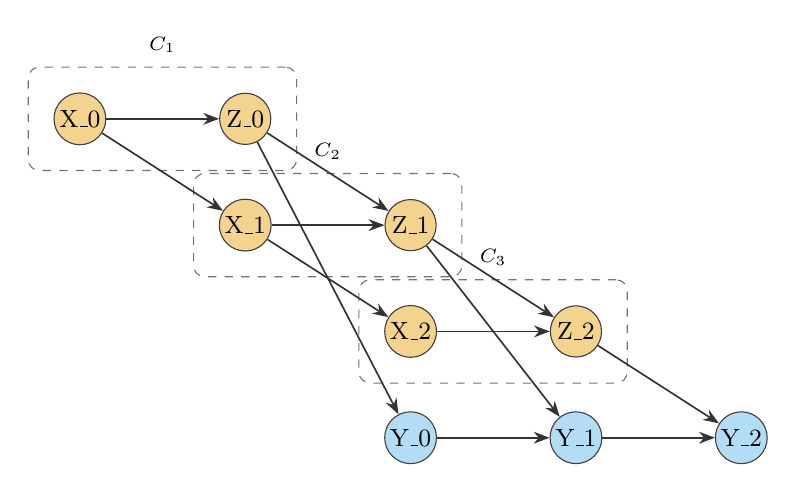
\begin{tikzpicture}
  \node[mannode] (nX0) at (0.00,0.00) {X\_0};
  \node[mannode] (nZ0) at (2.10,0.00) {Z\_0};
  \node[tgtnode] (nY0) at (4.20,-4.05) {Y\_0};
  \node[mannode] (nX1) at (2.10,-1.35) {X\_1};
  \node[mannode] (nZ1) at (4.20,-1.35) {Z\_1};
  \node[tgtnode] (nY1) at (6.30,-4.05) {Y\_1};
  \node[mannode] (nX2) at (4.20,-2.70) {X\_2};
  \node[mannode] (nZ2) at (6.30,-2.70) {Z\_2};
  \node[tgtnode] (nY2) at (8.40,-4.05) {Y\_2};
  \draw[diredge] (nX0) -- (nZ0);
  \draw[diredge] (nZ0) -- (nY0);
  \draw[diredge] (nX1) -- (nZ1);
  \draw[diredge] (nZ1) -- (nY1);
  \draw[diredge] (nX2) -- (nZ2);
  \draw[diredge] (nZ2) -- (nY2);
  \draw[diredge] (nX0) -- (nX1);
  \draw[diredge] (nZ0) -- (nZ1);
  \draw[diredge] (nY0) -- (nY1);
  \draw[diredge] (nX1) -- (nX2);
  \draw[diredge] (nZ1) -- (nZ2);
  \draw[diredge] (nY1) -- (nY2);
  \begin{scope}[on background layer]
    \node[clbox,fit=(nX0)(nZ0),label={[label distance=0.5mm]above:{\scriptsize$C_{1}$}}] {};
  \end{scope}
  \begin{scope}[on background layer]
    \node[clbox,fit=(nX1)(nZ1),label={[label distance=0.5mm]above:{\scriptsize$C_{2}$}}] {};
  \end{scope}
  \begin{scope}[on background layer]
    \node[clbox,fit=(nX2)(nZ2),label={[label distance=0.5mm]above:{\scriptsize$C_{3}$}}] {};
  \end{scope}
\end{tikzpicture}}\hfill
\adjustbox{max width=0.38\linewidth,valign=c}{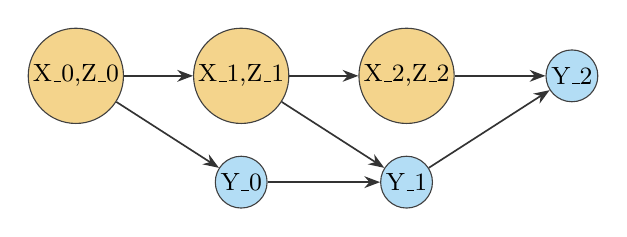
\begin{tikzpicture}
  \node[mannode] (nX0Z0) at (0.00,0.00) {X\_0,Z\_0};
  \node[tgtnode] (nY0) at (2.10,-1.35) {Y\_0};
  \node[mannode] (nX1Z1) at (2.10,0.00) {X\_1,Z\_1};
  \node[tgtnode] (nY1) at (4.20,-1.35) {Y\_1};
  \node[mannode] (nX2Z2) at (4.20,0.00) {X\_2,Z\_2};
  \node[tgtnode] (nY2) at (6.30,0.00) {Y\_2};
  \draw[diredge] (nX0Z0) -- (nY0);
  \draw[diredge] (nX1Z1) -- (nY1);
  \draw[diredge] (nX2Z2) -- (nY2);
  \draw[diredge] (nX0Z0) -- (nX1Z1);
  \draw[diredge] (nY0) -- (nY1);
  \draw[diredge] (nX1Z1) -- (nX2Z2);
  \draw[diredge] (nY1) -- (nY2);
\end{tikzpicture}}
\caption{\textbf{DCBO stat / nonstat (QDCBO family).} Fine DAG with coarse partition (left) and quotient C-DAG (right), in the convention of Fig.~\ref{fig:motivating}: manipulable variables orange, target blue, dash-dotted latent confounding; dashed boxes are the manipulable clusters. Slices $t=0,1,2$; the nonstat setup shares this topology with a change point in the SEM.}
\label{fig:dag-dcbo-stat}
\end{figure}

\begin{figure}[t]\centering
\adjustbox{max width=0.58\linewidth,valign=c}{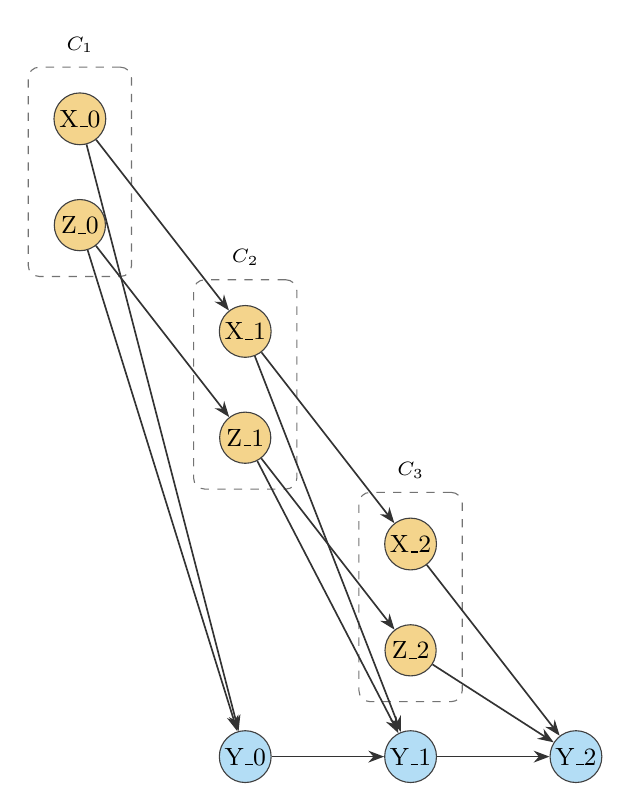
\begin{tikzpicture}
  \node[mannode] (nX0) at (0.00,0.00) {X\_0};
  \node[mannode] (nZ0) at (0.00,-1.35) {Z\_0};
  \node[tgtnode] (nY0) at (2.10,-8.10) {Y\_0};
  \node[mannode] (nX1) at (2.10,-2.70) {X\_1};
  \node[mannode] (nZ1) at (2.10,-4.05) {Z\_1};
  \node[tgtnode] (nY1) at (4.20,-8.10) {Y\_1};
  \node[mannode] (nX2) at (4.20,-5.40) {X\_2};
  \node[mannode] (nZ2) at (4.20,-6.75) {Z\_2};
  \node[tgtnode] (nY2) at (6.30,-8.10) {Y\_2};
  \draw[diredge] (nX0) -- (nY0);
  \draw[diredge] (nZ0) -- (nY0);
  \draw[diredge] (nX1) -- (nY1);
  \draw[diredge] (nZ1) -- (nY1);
  \draw[diredge] (nX2) -- (nY2);
  \draw[diredge] (nZ2) -- (nY2);
  \draw[diredge] (nX0) -- (nX1);
  \draw[diredge] (nZ0) -- (nZ1);
  \draw[diredge] (nY0) -- (nY1);
  \draw[diredge] (nX1) -- (nX2);
  \draw[diredge] (nZ1) -- (nZ2);
  \draw[diredge] (nY1) -- (nY2);
  \begin{scope}[on background layer]
    \node[clbox,fit=(nX0)(nZ0),label={[label distance=0.5mm]above:{\scriptsize$C_{1}$}}] {};
  \end{scope}
  \begin{scope}[on background layer]
    \node[clbox,fit=(nX1)(nZ1),label={[label distance=0.5mm]above:{\scriptsize$C_{2}$}}] {};
  \end{scope}
  \begin{scope}[on background layer]
    \node[clbox,fit=(nX2)(nZ2),label={[label distance=0.5mm]above:{\scriptsize$C_{3}$}}] {};
  \end{scope}
\end{tikzpicture}}\hfill
\adjustbox{max width=0.38\linewidth,valign=c}{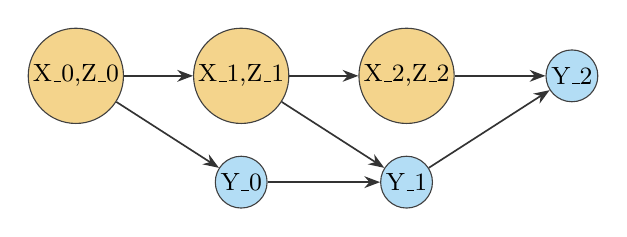
\begin{tikzpicture}
  \node[mannode] (nX0Z0) at (0.00,0.00) {X\_0,Z\_0};
  \node[tgtnode] (nY0) at (2.10,-1.35) {Y\_0};
  \node[mannode] (nX1Z1) at (2.10,0.00) {X\_1,Z\_1};
  \node[tgtnode] (nY1) at (4.20,-1.35) {Y\_1};
  \node[mannode] (nX2Z2) at (4.20,0.00) {X\_2,Z\_2};
  \node[tgtnode] (nY2) at (6.30,0.00) {Y\_2};
  \draw[diredge] (nX0Z0) -- (nY0);
  \draw[diredge] (nX1Z1) -- (nY1);
  \draw[diredge] (nX2Z2) -- (nY2);
  \draw[diredge] (nX0Z0) -- (nX1Z1);
  \draw[diredge] (nY0) -- (nY1);
  \draw[diredge] (nX1Z1) -- (nX2Z2);
  \draw[diredge] (nY1) -- (nY2);
\end{tikzpicture}}
\caption{\textbf{DCBO ind (QDCBO family).} Fine DAG with coarse partition (left) and quotient C-DAG (right), in the convention of Fig.~\ref{fig:motivating}: manipulable variables orange, target blue, dash-dotted latent confounding; dashed boxes are the manipulable clusters.}
\label{fig:dag-dcbo-ind}
\end{figure}

\begin{figure}[t]\centering
\adjustbox{max width=0.58\linewidth,valign=c}{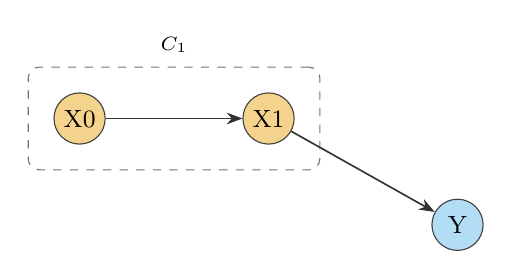
\begin{tikzpicture}
  \node[mannode] (nX0) at (0.00,0.00) {X0};
  \node[mannode] (nX1) at (2.40,0.00) {X1};
  \node[tgtnode] (nY) at (4.80,-1.35) {Y};
  \draw[diredge] (nX0) -- (nX1);
  \draw[diredge] (nX1) -- (nY);
  \begin{scope}[on background layer]
    \node[clbox,fit=(nX0)(nX1),label={[label distance=0.5mm]above:{\scriptsize$C_{1}$}}] {};
  \end{scope}
\end{tikzpicture}}\hfill
\adjustbox{max width=0.38\linewidth,valign=c}{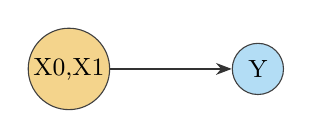
\begin{tikzpicture}
  \node[mannode] (nX0X1) at (0.00,0.00) {X0,X1};
  \node[tgtnode] (nY) at (2.40,0.00) {Y};
  \draw[diredge] (nX0X1) -- (nY);
\end{tikzpicture}}
\caption{\textbf{ToyGraph-M (QMCBO family).} Fine DAG with coarse partition (left) and quotient C-DAG (right), in the convention of Fig.~\ref{fig:motivating}: manipulable variables orange, target blue, dash-dotted latent confounding; dashed boxes are the manipulable clusters.}
\label{fig:dag-mcbo-toygraph-m}
\end{figure}

\begin{figure}[t]\centering
\adjustbox{max width=0.58\linewidth,valign=c}{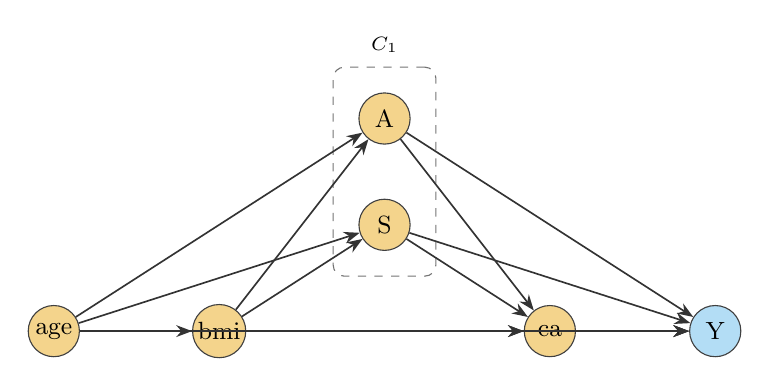
\begin{tikzpicture}
  \node[mannode] (nage) at (0.00,-2.70) {age};
  \node[mannode] (nbmi) at (2.10,-2.70) {bmi};
  \node[mannode] (nA) at (4.20,0.00) {A};
  \node[mannode] (nS) at (4.20,-1.35) {S};
  \node[mannode] (nca) at (6.30,-2.70) {ca};
  \node[tgtnode] (nY) at (8.40,-2.70) {Y};
  \draw[diredge] (nage) -- (nbmi);
  \draw[diredge] (nage) -- (nA);
  \draw[diredge] (nbmi) -- (nA);
  \draw[diredge] (nage) -- (nS);
  \draw[diredge] (nbmi) -- (nS);
  \draw[diredge] (nage) -- (nca);
  \draw[diredge] (nbmi) -- (nca);
  \draw[diredge] (nA) -- (nca);
  \draw[diredge] (nS) -- (nca);
  \draw[diredge] (nage) -- (nY);
  \draw[diredge] (nbmi) -- (nY);
  \draw[diredge] (nA) -- (nY);
  \draw[diredge] (nS) -- (nY);
  \draw[diredge] (nca) -- (nY);
  \begin{scope}[on background layer]
    \node[clbox,fit=(nA)(nS),label={[label distance=0.5mm]above:{\scriptsize$C_{1}$}}] {};
  \end{scope}
\end{tikzpicture}}\hfill
\adjustbox{max width=0.38\linewidth,valign=c}{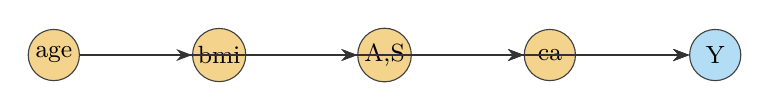
\begin{tikzpicture}
  \node[mannode] (nage) at (0.00,0.00) {age};
  \node[mannode] (nbmi) at (2.10,0.00) {bmi};
  \node[mannode] (nAS) at (4.20,0.00) {A,S};
  \node[mannode] (nca) at (6.30,0.00) {ca};
  \node[tgtnode] (nY) at (8.40,0.00) {Y};
  \draw[diredge] (nage) -- (nbmi);
  \draw[diredge] (nage) -- (nAS);
  \draw[diredge] (nbmi) -- (nAS);
  \draw[diredge] (nage) -- (nca);
  \draw[diredge] (nbmi) -- (nca);
  \draw[diredge] (nAS) -- (nca);
  \draw[diredge] (nage) -- (nY);
  \draw[diredge] (nbmi) -- (nY);
  \draw[diredge] (nAS) -- (nY);
  \draw[diredge] (nca) -- (nY);
\end{tikzpicture}}
\caption{\textbf{PSAGraph (QMCBO family).} Fine DAG with coarse partition (left) and quotient C-DAG (right), in the convention of Fig.~\ref{fig:motivating}: manipulable variables orange, target blue, dash-dotted latent confounding; dashed boxes are the manipulable clusters.}
\label{fig:dag-mcbo-psagraph}
\end{figure}


\endgroup
\clearpage

\end{document}
